
%--- 幻灯片1:提纲 ---
\begin{refsection}
  \begin{frame}{提纲}
    \begin{itemize}
      \item 1. 基于深度学习的图像分类简介
      \item 2. 传统数据增强方法
      \item 3. 用于数据增强的生成模型
      \item 4. 灾害事件遥感数据集:xBD
    \end{itemize}
    \begin{itemize}
      \item 项目 - \textbf{探索生成图像是否能提升图像分类效果}
    \end{itemize}
  \end{frame}
\end{refsection}

\begin{refsection}
  \begin{frame}{图像分类:概述}
    \begin{figure}
      \centering
      \includegraphics[height=0.6\textheight]{image_classification_idea.png}
      \caption{\scriptsize 图像分类概述。}
    \end{figure}
    \bottomleftrefs
  \end{frame}
\end{refsection}

\begin{refsection}
  \begin{frame}{背景:深度学习下的图像分类}
    \begin{figure}
      \centering
      \begin{minipage}{0.48\linewidth}
        \centering
        \includegraphics[width=\linewidth]{imagenet2.png}
      \end{minipage}\hfill
      \begin{minipage}{0.48\linewidth}
        \centering
        \includegraphics[width=\linewidth]{alexnet.png}
      \end{minipage}
      \caption[]{\scriptsize 左:ILSVRC-2010上的AlexNet~\parencite{imagenet2010challenge} \quad 右:AlexNet结构~\parencite{krizhevskyImageNetClassificationDeep2012}。}
    \end{figure}
    \bottomleftrefs
  \end{frame}
\end{refsection}

\begin{refsection}
  \begin{frame}{图像分类架构演进}
    \begin{minipage}{0.48\linewidth}
      {\small
      \begin{itemize}
        \item \textbf{2012: AlexNet}, \textbf{2016: ResNet}
        \item \textbf{2021: ViT} \\
        \parencite{dosovitskiyImageWorth16x162020}
        \item \textbf{2021: Swin Transformer} \\
        \parencite{liuSwinTransformerHierarchical2021}
        \item \textbf{2021: CLIP-ViT} \\
        \parencite{radfordLearningTransferableVisual2021}
        \item \textbf{2022: MAE-ViT} \\
        \parencite{heMaskedAutoencodersAre2022}
        \item \textbf{2022: CoCa-ViT} \\
        \parencite{yuCoCaContrastiveCaptioners2022}
      \end{itemize}
      }
    \end{minipage}%
    \hfill
    \begin{minipage}{0.48\linewidth}
      \centering
      \includegraphics[width=0.95\linewidth]{vit.png}
      \scriptsize Vision Transformer结构概览\\\parencite{dosovitskiyImageWorth16x162020}。
    \end{minipage}
    \bottomleftrefs
  \end{frame}
\end{refsection}

% \begin{refsection}
%   \begin{frame}{RemoteCLIP: Vision-Language Foundation Model for Remote Sensing}
%     \begin{figure}
%       \centering
%       \includegraphics[width=0.8\linewidth]{remoteclip.png}
%       \caption{\scriptsize RemoteCLIP~\parencite{liuRemoteCLIPVisionLanguage2024}: A Vision-Language Foundation Model for Remote Sensing.}
%     \end{figure}
%     \bottomleftrefs
%   \end{frame}
% \end{refsection}

\begin{refsection}
  \begin{frame}{图像分类数据集:RESISC45}
    \begin{figure}
      \centering
      \includegraphics[width=0.7\linewidth]{RESISC45_part.png}
    \end{figure}
    \scriptsize
    RESISC45遥感场景分类数据集示例图像~\parencite{Cheng2017}。
    \bottomleftrefs
  \end{frame}
\end{refsection}

\begin{refsection}
  \begin{frame}{传统数据增强方法}
    \begin{itemize}
      \item \textbf{几何变换:} \textbf{旋转}、\textbf{翻转}(水平/垂直)、\textbf{缩放}、\textbf{平移}、\textbf{裁剪}
      \item \textbf{颜色扰动:} 调整亮度、对比度、饱和度和色调
      \item \textbf{噪声注入:} 向图像中添加随机噪声
      \item \textbf{Cutout}~\parencite{devriesImprovedRegularizationConvolutional2017}
      \item \textbf{CutMix}~\parencite{yunCutMixRegularizationStrategy2019}
      \item \textbf{Copy-Paste}~\parencite{ghiasiSimpleCopyPasteStrong2021}
    \end{itemize}
    还有一项综合研究《How to train your ViT? Data, Augmentation,  and Regularization in Vision Transformers》~\parencite{steinerHowTrainYour2022}。
    \bottomleftrefs
  \end{frame}
\end{refsection}

\begin{refsection}
  \begin{frame}{用于数据增强的生成模型}
    \begin{minipage}{0.7\linewidth}
      \includegraphics[width=0.9\linewidth]{satsyn.png}
    \end{minipage}%
    \hfill
    \begin{minipage}{0.3\linewidth}
      \scriptsize
      SatSyn~\parencite{tokerSatSynthAugmentingImageMask2024} 提出了一种生成模型(扩散模型),可同时生成卫星分割的图像和对应掩码。该合成数据集用于数据增强,在卫星语义分割任务中相比其他增强方法带来了显著的定量提升。
    \end{minipage}
    \bottomleftrefs
  \end{frame}
\end{refsection}

\begin{refsection}
  \begin{frame}{生成的文本-图像数据集提升图像分类}
    \centering
    \includegraphics[width=0.8\linewidth]{syn_aug_results.png}
    
    \scriptsize
    由生成模型合成的文本-图像数据集可以显著提升图像分类性能,如~\parencite{heSYNTHETICDATAGENERATIVE2022}所示。
    \bottomleftrefs
  \end{frame}
\end{refsection}

\begin{refsection}
  \begin{frame}{xBD:大规模灾害损失数据集}
    \centering
    \includegraphics[width=0.85\linewidth]{xbd_samples.png}
    
    \vspace{0.5em}
    \scriptsize
    灾前影像(上)与灾后影像(下)。从左到右依次为:哈维飓风、乔普林龙卷风、下普纳火山喷发、巽他海峡海啸。影像来源:DigitalGlobe。\\
    \textbf{xBD}~\parencite{guptaCreatingXBDDataset2019}
    \bottomleftrefs
  \end{frame}
\end{refsection}

\begin{refsection}
  \begin{frame}{xBD:全球灾害类型覆盖}
    \centering
    \includegraphics[width=0.85\linewidth]{xbd_global.png}
    
    \vspace{0.5em}
    \scriptsize
    xBD数据集在全球范围内涵盖的灾害类型及事件。\\
    \textbf{xBD}~\parencite{guptaCreatingXBDDataset2019}
    \bottomleftrefs
  \end{frame}
\end{refsection}

\begin{refsection}
  \begin{frame}{项目作业:总体介绍}
    \textbf{项目:生成图像能否提升遥感图像分类?}
  
    \vspace{0.7em}
    \textbf{目标:}\\
    探索将真实图像与生成图像结合,是否能提升遥感图像分类效果。

    \vspace{1em}
    \textbf{实验流程:}\\
    本项目将通过三种不同训练设置,评估生成数据的影响:
    \begin{enumerate}
      \item \textbf{仅用真实数据集:} 仅用xBD数据集中的真实图像训练分类模型。
      \item \textbf{仅用生成数据集:} 仅用商业生成模型合成的图像训练模型。
      \item \textbf{真实+生成数据集:} 同时用真实图像和生成图像训练模型。
    \end{enumerate}
    比较三种设置下的分类性能,分析合成数据的作用。

    \bottomleftrefs
  \end{frame}
\end{refsection}
  
%--- 幻灯片:数据集 ---
\begin{refsection}
  \begin{frame}{项目作业:数据集}
    \textbf{数据集:xBD灾害损失数据集}
    \begin{itemize}
      \item 使用\textbf{xBD}遥感灾害数据集。
      \item 数据集包含\textbf{6类灾害}。
      \item 每类灾害选取\textbf{100张真实图像}(共600张真实图像)。
    \end{itemize}
    \bottomleftrefs
  \end{frame}
  \end{refsection}
  
  %--- 幻灯片:生成模型 ---
  \begin{refsection}
    \begin{frame}{项目作业:生成模型}
      \textbf{图像生成:}
      \begin{itemize}
        \item 生成图像视为\textbf{文本引导的图像编辑}结果:每个案例输入\textbf{灾前图像}和\textbf{文本描述}(如“洪水”、“建筑倒塌”),模型生成灾后图像。
        \item 可使用商业生成模型,如\textbf{GPT-4o图像生成(GPT-Image-1)}~\parencite{gptimage1}、\textbf{Gemini-2}~\parencite{gemini2}或\textbf{SeedEdit 3.0}~\parencite{wang2025seedit},为每类灾害生成合成图像。
      \end{itemize}
      \bottomleftrefs
    \end{frame}
  \end{refsection}
  
  %--- 幻灯片:分类模型 ---
  \begin{refsection}
  \begin{frame}{项目作业:分类模型}
    \textbf{推荐基线模型:}
    \begin{itemize}
      \item \textbf{OpenAI CLIP}~\parencite{radfordLearningTransferableVisual2021}~\href{https://hf-mirror.com/openai/clip-vit-base-patch16}{\textcolor{blue}{- 模型}}
      \item \textbf{RemoteCLIP}~\parencite{liuRemoteCLIPVisionLanguage2024}~\href{https://hf-mirror.com/MVRL/remote-clip-vit-base-patch32}{\textcolor{blue}{- 模型}}
      \item \textbf{Git-RSCLIP}~\parencite{text2earth2025}~\href{https://hf-mirror.com/lcybuaa/Git-RSCLIP-base}{\textcolor{blue}{- 模型}}
    \end{itemize}
    \vspace{0.5em}
    以上模型均为ViT结构。代码与教程参考:
    \begin{itemize}
      \item \href{https://github.com/huggingface/transformers/blob/main/examples/pytorch/contrastive-image-text/README.md}{\textcolor{blue}{CLIP训练示例}}
      \item \href{https://github.com/NielsRogge/Transformers-Tutorials/tree/master/VisionTransformer}{\textcolor{blue}{ViT教程}}
      \item 更多遥感基础模型见~\href{https://hf-mirror.com/collections/MVRL/remote-sensing-foundation-models-664e8fcd67d8ca8c03f42d00}{\textcolor{purple}{huggingface合集}}
    \end{itemize}
    \bottomleftrefs
  \end{frame}
  \end{refsection}
  
  %--- 幻灯片:数据增强方案 ---
  \begin{refsection}
  \begin{frame}{项目作业:数据增强方案}
    \begin{itemize}
      \item 每类灾害生成\textbf{1$\times$--4$\times$}数量的合成图像(即每类100、200、300或400张合成图像)。
      \item 探索并比较不同真实与合成图像比例(如1:1、1:2、1:3、1:4)。
      \item 每类灾害增强后数据集规模为\textbf{200到500张}。
    \end{itemize}
    \bottomleftrefs
  \end{frame}
  \end{refsection}
  
  %--- 幻灯片:评估 ---
  \begin{refsection}
  \begin{frame}{项目作业:评估}
    \textbf{评估方式:}
    \begin{itemize}
      \item 使用\textbf{标准准确率}、\textbf{F1分数}和\textbf{混淆矩阵}衡量性能。
      \item 始终在\textbf{保留的真实(未见过的)测试集}上评估。
      \item 绘制\textbf{曲线或柱状图},比较不同真实:合成比例下的分类性能。
    \end{itemize}
    \bottomleftrefs
  \end{frame}
  \end{refsection}
  

% \begin{refsection}
%   \begin{frame}{Baseline Models for Scene Classification}
%     \textbf{Scene Image Classification:}
%     \begin{itemize}
%       \item \textbf{OpenAI CLIP}~\parencite{radfordLearningTransferableVisual2021}~\href{https://hf-mirror.com/openai/clip-vit-base-patch16}{\textcolor{blue}{- models}}
%       \item \textbf{RemoteCLIP}~\parencite{liuRemoteCLIPVisionLanguage2024}~\href{https://hf-mirror.com/MVRL/remote-clip-vit-base-patch32}{\textcolor{blue}{- models}}
%       \item \textbf{Git-RSCLIP}~\parencite{text2earth2025}~\href{https://hf-mirror.com/lcybuaa/Git-RSCLIP-base}{\textcolor{blue}{- models}}
%     \end{itemize}
%     All of above follow ViT configuration where we can use following~\href{https://github.com/huggingface/transformers/blob/main/examples/pytorch/contrastive-image-text/README.md}{\textcolor{blue}{(code)}}~for continuing CLIP training or ~\href{https://github.com/NielsRogge/Transformers-Tutorials/tree/master/VisionTransformer}{\textcolor{blue}{(code)}}~ for fine-tuning on classification task.
%     For more Remote Sensing Foundation Models, ref to ~\href{https://hf-mirror.com/collections/MVRL/remote-sensing-foundation-models-664e8fcd67d8ca8c03f42d00}{\textcolor{purple}{huggingface collection}.}
%     \bottomleftrefs
%   \end{frame}
%   \end{refsection}



\begin{refsection}
  \begin{frame}[plain]
    \vfill
    \centering
    {\Huge \textbf{附录}}
    \vfill
  \end{frame}
\end{refsection}

  %--- 幻灯片:文本到图像生成的数据集 ---
  \begin{refsection}
    \begin{frame}{更多文本-图像遥感数据集}
      \textbf{文本到图像生成:}
      \begin{itemize}
        \item \textbf{RSICD}~\parencite{lu2017exploring}:遥感图像描述数据集,含10,921张图像,每张配有5条描述。
        \item \textbf{RSICap}~\parencite{hu2023rsgpt}:高质量数据集,包含2,585个人工标注的图像-描述对。
        \item \textbf{UCM-Captions}~\parencite{qu2016deep}:基于UC Merced土地利用数据集,含2,100张图像,每张配5条描述。
        \item \textbf{RESISC45}~\parencite{Cheng2017}:公开的遥感场景分类基准数据集,由西北工业大学创建,共31,500张图像,覆盖45类场景,每类700张。
      \end{itemize}
      \bottomleftrefs
    \end{frame}
  \end{refsection}

\begin{refsection}
  \begin{frame}{生成建模}
    \begin{figure}
      \centering
      \includegraphics[width=0.8\linewidth]{learning_to_generate_data.png}
      \caption{\scriptsize 生成建模示意图~\parencite{CVPR2023Tutorial}。}
    \end{figure}
    \bottomleftrefs
  \end{frame}
  \end{refsection}
  
  % --- 幻灯片2:生成模型发展时间线 ---
  \begin{refsection}
  \begin{frame}{生成模型发展时间线}
    \begin{figure}
      \centering
      \includegraphics[width=0.95\linewidth]{genai_timeline.png}
      \caption{\scriptsize 生成模型关键进展时间线~\parencite{dengPPTAdvancedNueralNetwork2024}。}
    \end{figure}
    \bottomleftrefs
  \end{frame}
  \end{refsection}
  
  
  
  \begin{refsection}
  \begin{frame}{背景:扩散模型}
  
    \begin{figure}
      \begin{minipage}{0.95\linewidth}
        \footnotesize
        \textbf{去噪扩散模型包含两个过程:}
        \begin{itemize}
          \item 正向扩散过程:逐步向输入添加噪声。
          \item 反向去噪过程:通过去噪学习生成数据。
        \end{itemize}
      \end{minipage}
      \vspace{2em}
  
      \centering
      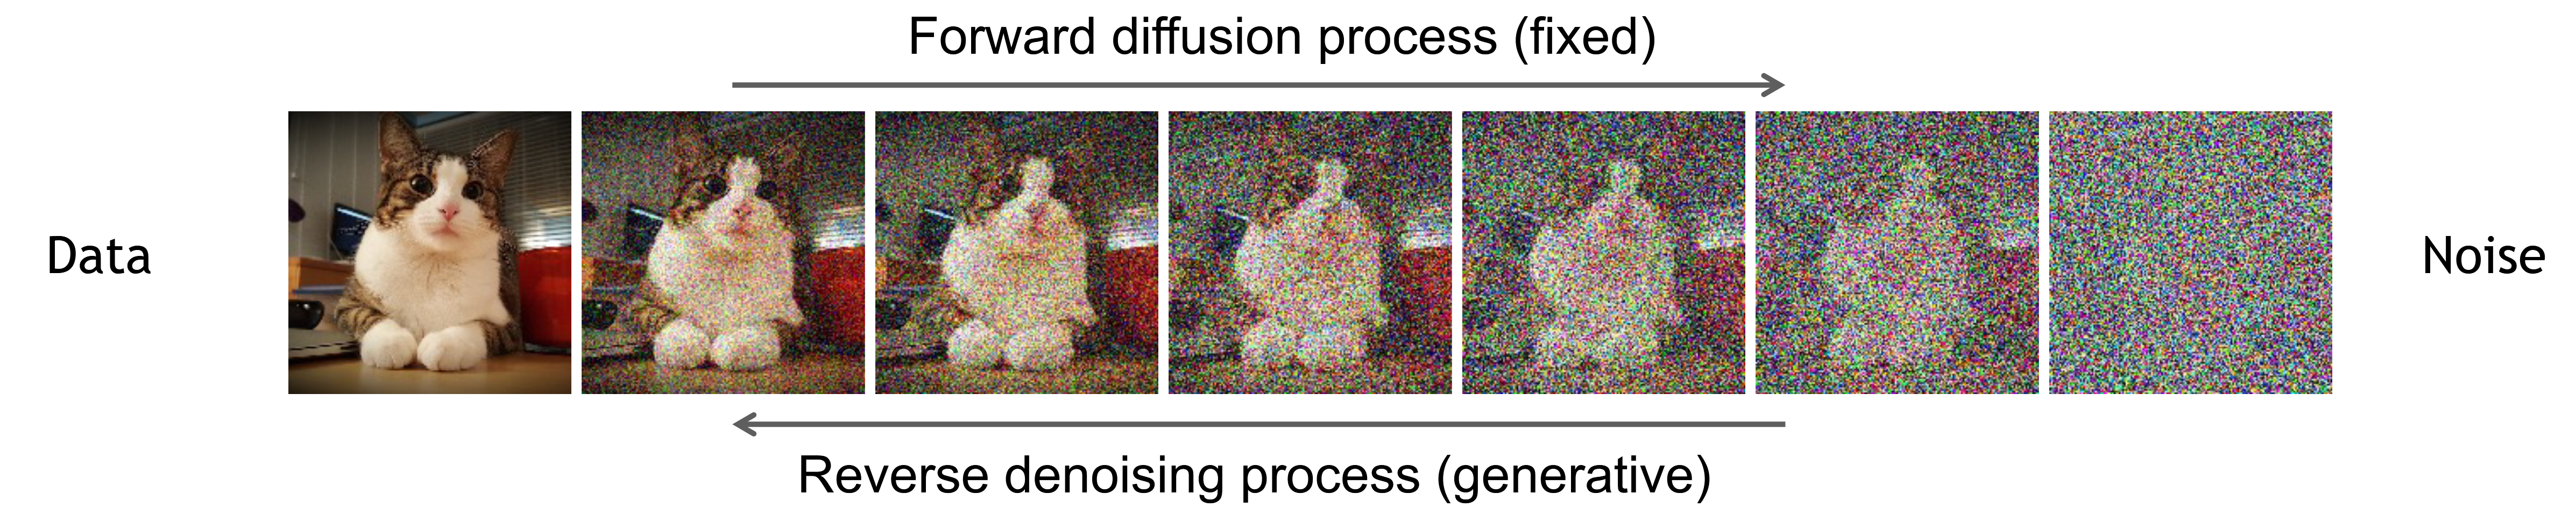
\includegraphics[width=1.0\linewidth]{diffusion_high_level.png}
  
      \caption[]{\scriptsize 扩散模型通过迭代去噪生成数据~\parencite{sohl2015deep,ho2020denoising}。}
    \end{figure}
  
    \bottomleftrefs
  \end{frame}
  \end{refsection}
  
  % --- 幻灯片4:扩散模型原理 ---
  \begin{refsection}
  \begin{frame}{扩散模型:正向与反向过程}
    \footnotesize
    \textbf{正向(扩散)过程:}
    \begin{align*}
      q(\mathbf{x}_t \mid \mathbf{x}_{t-1}) &= \mathcal{N}(\mathbf{x}_t; \sqrt{1-\beta_t}\,\mathbf{x}_{t-1}, \beta_t \mathbf{I}) \\
      q(\mathbf{x}_{1:T} \mid \mathbf{x}_0) &= \prod_{t=1}^T q(\mathbf{x}_t \mid \mathbf{x}_{t-1}) \\
      &\text{等价于} 
      \mathbf{x}_t = \sqrt{\bar{\alpha}_t}\,\mathbf{x}_0 + \sqrt{1-\bar{\alpha}_t}\,\boldsymbol{\epsilon}, \quad \boldsymbol{\epsilon} \sim \mathcal{N}(\mathbf{0}, \mathbf{I})
    \end{align*}
  
    \footnotesize
    \textbf{反向(去噪)过程:}
    \begin{align*}
      p_\theta(\mathbf{x}_{t-1} \mid \mathbf{x}_t) &= \mathcal{N}(\mathbf{x}_{t-1}; \boldsymbol{\mu}_\theta(\mathbf{x}_t, t), \Sigma_\theta(\mathbf{x}_t, t)) \\
      p_\theta(\mathbf{x}_{0:T}) &= p(\mathbf{x}_T) \prod_{t=1}^T p_\theta(\mathbf{x}_{t-1} \mid \mathbf{x}_t)
    \end{align*}
    \scriptsize
    其中$\mathbf{x}_0$为数据,$\beta_t$为噪声调度,$\bar{\alpha}_t = \prod_{s=1}^t (1-\beta_s)$,$p(\mathbf{x}_T) = \mathcal{N}(\mathbf{0}, \mathbf{I})$。
  
    \scriptsize
    \textbf{扩散模型通过学习逆转逐步加噪过程来生成数据。}~\parencite{sohl2015deep,ho2020denoising}
    \bottomleftrefs
  \end{frame}
  \end{refsection}
  
  \begin{refsection}
  \begin{frame}{扩散模型:训练与推理}
    \footnotesize
    \textbf{训练目标:}
    \begin{align*}
      \mathcal{L}_{\mathrm{simple}} = \mathbb{E}_{\mathbf{x}_0, \boldsymbol{\epsilon}, t} \left[ \left\| \boldsymbol{\epsilon} - \boldsymbol{\epsilon}_\theta(\sqrt{\bar{\alpha}_t}\mathbf{x}_0 + \sqrt{1-\bar{\alpha}_t}\boldsymbol{\epsilon}, t) \right\|^2 \right]
    \end{align*}
    其中$\boldsymbol{\epsilon} \sim \mathcal{N}(\mathbf{0}, \mathbf{I})$,$\bar{\alpha}_t = \prod_{s=1}^t (1-\beta_s)$。
  
    \vspace{0.5em}
    \textbf{推理(采样):}
    \begin{itemize}
      \item 从纯噪声开始:$\mathbf{x}_T \sim \mathcal{N}(\mathbf{0}, \mathbf{I})$
      \item 对于$t = T, \ldots, 1$:
        \begin{itemize}
          \item 预测噪声:$\boldsymbol{\epsilon}_\theta(\mathbf{x}_t, t)$
          \item 计算均值:$\boldsymbol{\mu}_\theta(\mathbf{x}_t, t)$
          \item 采样:$\mathbf{x}_{t-1} \sim \mathcal{N}(\boldsymbol{\mu}_\theta(\mathbf{x}_t, t), \Sigma_\theta(\mathbf{x}_t, t))$
        \end{itemize}
      \item 重复直到$\mathbf{x}_0$(生成样本)
    \end{itemize}
  
    \vspace{0.5em}
    \scriptsize
    \textbf{训练:} 最小化简化目标~\parencite{ho2020denoising}。\\
    \textbf{推理:} 通过迭代去噪从随机噪声生成数据。
    \bottomleftrefs
  \end{frame}
  \end{refsection}
  
  %--- 幻灯片5:遥感图像生成应用:DiffusionSat, CRS-Diff, Text2Earth ---
  
  \begin{refsection}
    \begin{frame}{遥感图像生成应用:Text2Earth}
      \begin{figure}
        \centering
        \includegraphics[width=0.9\linewidth]{text2earth.png}
        \caption[]{\scriptsize Text2Earth:面向文本驱动地球观测的基础模型~\parencite{text2earth2025}。}
      \end{figure}
      \bottomleftrefs
    \end{frame}
  \end{refsection}
  
  \begin{refsection}
    \begin{frame}{Text2Earth:示例结果}
      \begin{figure}
        \centering
        \includegraphics[width=0.9\linewidth]{text2earth_results.png}
        \caption[]{\scriptsize Text2Earth生成的示例结果~\parencite{text2earth2025}。}
      \end{figure}
      \bottomleftrefs
    \end{frame}
  \end{refsection}
  
  \begin{refsection}
  \begin{frame}{遥感图像生成应用:CRS-Diff}
    \begin{figure}
      \centering
      \includegraphics[width=0.9\linewidth]{crsdiff.png}
      \caption[]{\scriptsize CRS-Diff:可控遥感图像生成框架~\parencite{tang2024crsdiff}。}
    \end{figure}
    \bottomleftrefs
  \end{frame}
  \end{refsection}
  
  \begin{refsection}
  \begin{frame}{CRS-Diff:示例结果}
    \begin{figure}
      \centering
      \includegraphics[width=0.9\linewidth]{crsdiff_results.png}
      \caption[]{\scriptsize CRS-Diff生成的示例结果~\parencite{tang2024crsdiff}。}
    \end{figure}
    \bottomleftrefs
  \end{frame}
  \end{refsection}
  
  %--- 幻灯片6a:DiffusionSat框架 ---
  \begin{refsection}
  \begin{frame}{DiffusionSat:框架概览}
    \begin{figure}
      \centering
      \includegraphics[width=0.9\linewidth]{diffusionsat.png}
      \caption[]{\scriptsize DiffusionSat:卫星影像生成基础模型~\parencite{diffusionset2024}。}
    \end{figure}
    \bottomleftrefs
  \end{frame}
  \end{refsection}
  
  %--- 幻灯片6b:DiffusionSat超分辨率 ---
  \begin{refsection}
  \begin{frame}{DiffusionSat:超分辨率结果}
    \begin{figure}
      \centering
      \includegraphics[width=0.9\linewidth]{diffusionsat_sr_results.png}
      \caption[]{\scriptsize DiffusionSat多光谱超分辨率示例结果~\parencite{diffusionset2024}。}
    \end{figure}
    \bottomleftrefs
  \end{frame}
  \end{refsection}
  
  %--- 幻灯片6c:DiffusionSat修复 ---
  \begin{refsection}
  \begin{frame}{DiffusionSat:修复结果}
    \begin{figure}
      \centering
      \includegraphics[width=0.9\linewidth]{diffusionsat_inpainting_results.png}
      \caption[]{\scriptsize DiffusionSat遥感图像修复示例结果~\parencite{diffusionset2024}。}
    \end{figure}
    \bottomleftrefs
  \end{frame}
  \end{refsection}
